% ==============================================================================
% SkinWise AI — Rapport Technique (version simplifiée)
% Compiler avec : pdflatex rapport_technique.tex (2 fois)
% Les figures sont dans le dossier figures/
% ==============================================================================
\documentclass[11pt,a4paper]{report}

\usepackage[utf8]{inputenc}
\usepackage[T1]{fontenc}
\usepackage[french]{babel}
\usepackage[top=2.5cm,bottom=2.5cm,left=2.5cm,right=2.5cm]{geometry}
\usepackage{graphicx}
\usepackage{float}
\usepackage{booktabs}
\usepackage[table]{xcolor}
\usepackage{listings}
\usepackage{hyperref}
\usepackage{enumitem}
\usepackage{fancyhdr}
\usepackage{mdframed}
\usepackage{array}
\usepackage{titlesec}
\usepackage{tikz}
\usetikzlibrary{arrows.meta,positioning,fit,backgrounds}

\graphicspath{{figures/}}

% ----------------------------- Couleurs ---------------------------------------
\definecolor{codebg}{RGB}{248,250,252}
\definecolor{codeframe}{RGB}{203,213,225}
\definecolor{tekupblue}{RGB}{26,86,219}
\definecolor{resultbg}{RGB}{239,246,255}
\definecolor{resultborder}{RGB}{147,197,253}
\definecolor{darkblue}{RGB}{25,55,150}
\definecolor{warnbg}{RGB}{255,247,237}
\definecolor{warnborder}{RGB}{251,146,60}

\hypersetup{colorlinks=true, linkcolor=darkblue, urlcolor=darkblue, citecolor=darkblue,
            pdftitle={SkinWise AI — Rapport Technique}, pdfauthor={Hedi Laifa}}

% ----------------------------- En-tête / Pied de page ------------------------
\pagestyle{fancy}
\fancyhf{}
\fancyhead[L]{\small\textit{SkinWise AI — Classification de la sévérité de l'acné}}
\fancyhead[R]{\small\textbf{TEK-UP}}
\fancyfoot[C]{\thepage}
\renewcommand{\headrulewidth}{0.4pt}
\setlength{\headheight}{14pt}

\titleformat{\chapter}[display]{\normalfont\huge\bfseries}{\Large\chaptertitlename\ \thechapter}{12pt}{\Huge}
\titlespacing*{\chapter}{0pt}{-10pt}{25pt}

% ----------------------------- Boîtes ----------------------------------------
\newmdenv[backgroundcolor=resultbg, linecolor=resultborder, linewidth=1.5pt, roundcorner=4pt,
  innertopmargin=8pt, innerbottommargin=8pt, innerleftmargin=10pt, innerrightmargin=10pt,
  skipabove=10pt, skipbelow=6pt]{resultatcle}
\newmdenv[backgroundcolor=warnbg, linecolor=warnborder, linewidth=1.5pt, roundcorner=4pt,
  innertopmargin=8pt, innerbottommargin=8pt, innerleftmargin=10pt, innerrightmargin=10pt,
  skipabove=10pt, skipbelow=6pt]{limite}

% ----------------------------- Code ------------------------------------------
\lstset{backgroundcolor=\color{codebg}, frame=single, rulecolor=\color{codeframe},
        basicstyle=\ttfamily\footnotesize, breaklines=true, showstringspaces=false,
        captionpos=b, columns=fullflexible,
        literate={é}{{\'e}}1 {è}{{\`e}}1 {à}{{\`a}}1 {ê}{{\^e}}1 {î}{{\^i}}1 {ô}{{\^o}}1 {â}{{\^a}}1 {ù}{{\`u}}1 {ç}{{\c{c}}}1 {É}{{\'E}}1 {→}{{$\rightarrow$}}1}

\begin{document}

% ==============================================================================
%                              PAGE DE COUVERTURE
% ==============================================================================
\begin{titlepage}
\centering
{\Large\textbf{TEK-UP}}\\[0.2em]
{\normalsize École Supérieure Privée}\\
{\normalsize Technologie \& Ingénierie}

\vspace{1.5cm}
\hrule height 0.5pt
\vspace{0.3cm}
{\small\scshape Projet de Module — Deep Learning Avancé \& MLOps}\\[0.2em]
{\small Cycle Ingénieur en Intelligence Artificielle \& Data Science — 3\textsuperscript{ème} année}
\vspace{0.3cm}
\hrule height 0.5pt

\vspace{2cm}
{\fontsize{22}{28}\selectfont\bfseries
SkinWise AI\\[0.5em]
Classification automatique\\[0.3em]
de la sévérité de l'acné
}

\vspace{1.2cm}
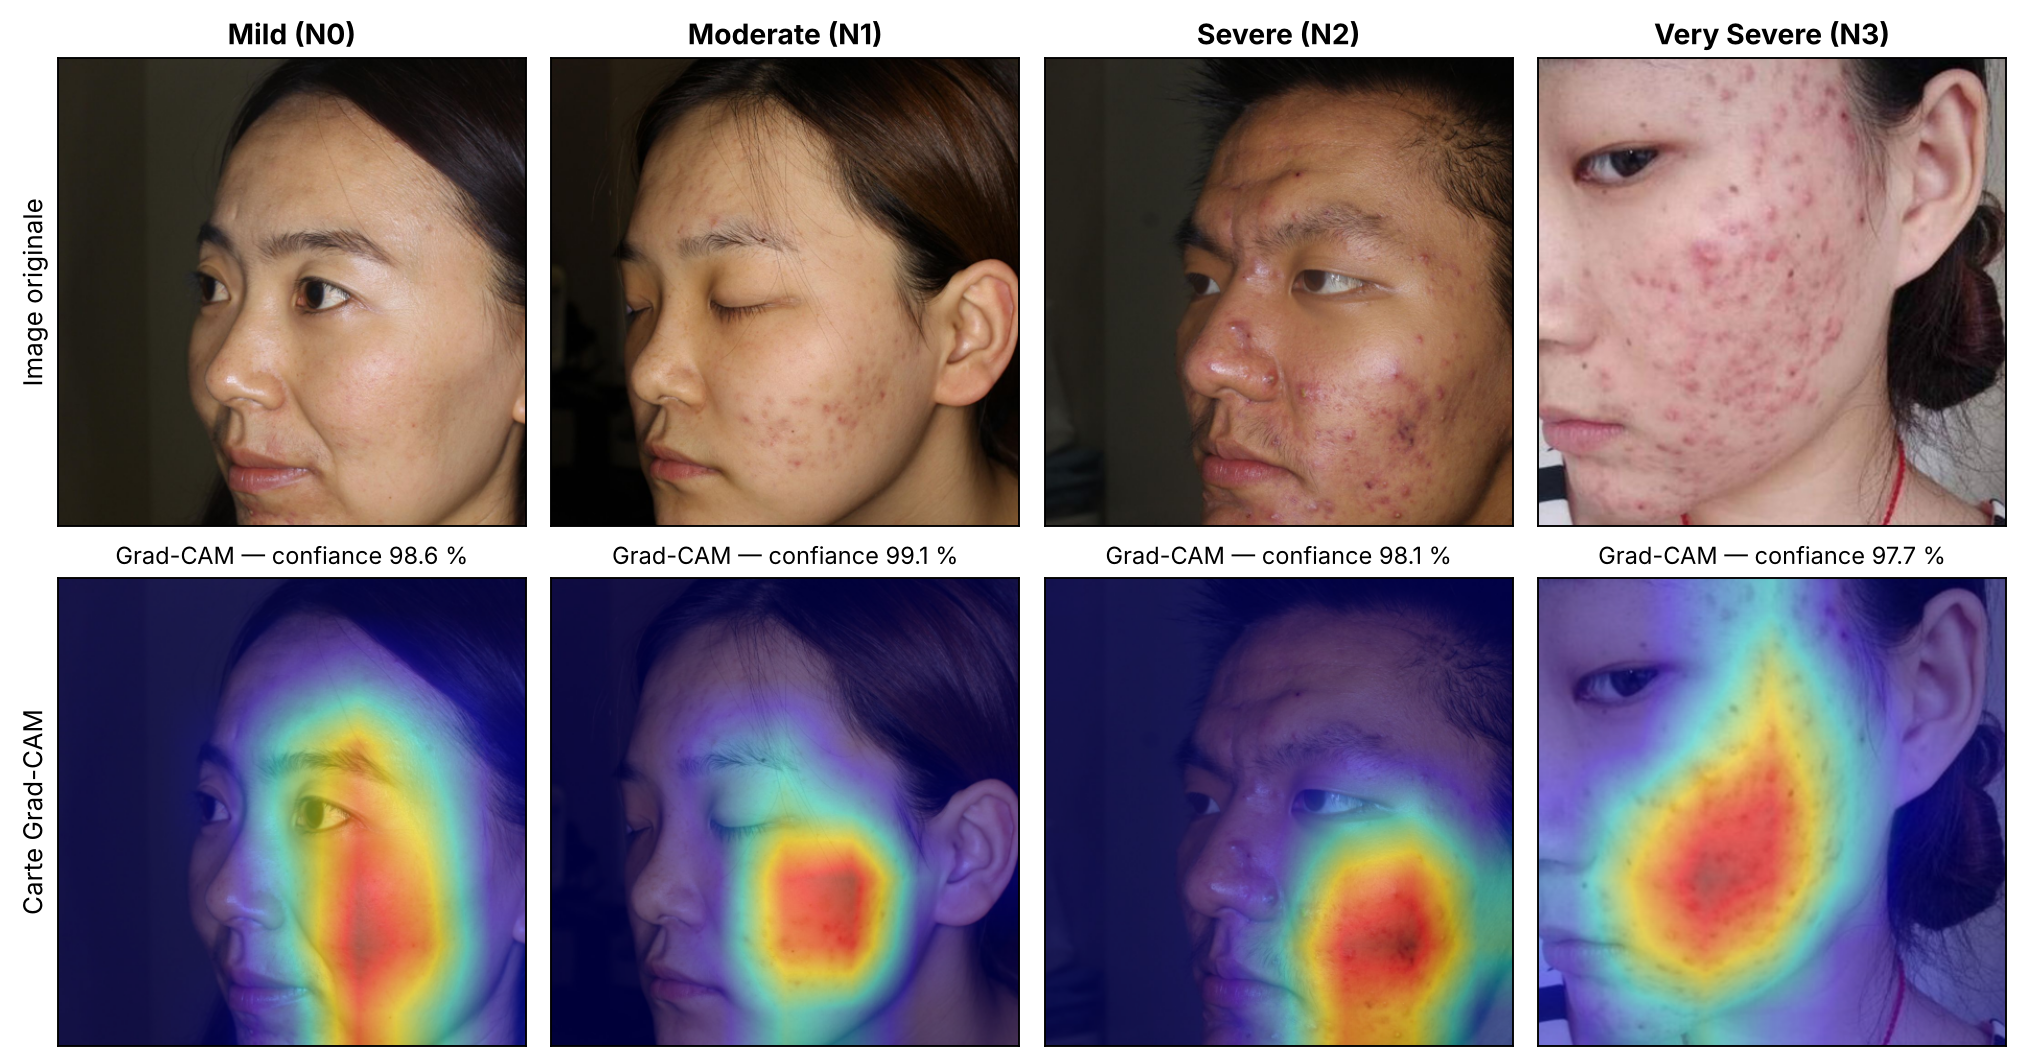
\includegraphics[width=0.85\textwidth]{gradcam_grid.png}

\vspace{1.2cm}
\hrule height 0.5pt
\vspace{0.5cm}
\begin{minipage}[t]{0.45\textwidth}
\raggedright
\textit{Réalisé par :}\\[0.4em]
\textbf{Hedi Laifa}\\
Cycle Ingénieur IA \& Data Science\\
3\textsuperscript{ème} année
\end{minipage}
\hfill
\begin{minipage}[t]{0.45\textwidth}
\raggedleft
\textit{Encadré par :}\\[0.4em]
\textbf{M. Haythem Ghazouani}\\
Module Deep Learning Avancé\\
TEK-UP
\end{minipage}

\vfill
{\large Année universitaire 2026--2027}
\end{titlepage}

\tableofcontents
\newpage

% ==============================================================================
\chapter*{Introduction}
\addcontentsline{toc}{chapter}{Introduction}
\markboth{Introduction}{Introduction}

L'acné est l'une des maladies de peau les plus fréquentes, surtout chez les jeunes. Pour
choisir un traitement, un dermatologue évalue d'abord sa \textbf{sévérité}. Cette évaluation
se fait à l'œil et peut varier d'un médecin à l'autre.

\medskip
Dans ce projet, nous avons construit \textbf{SkinWise AI} : une application web qui reçoit
la photo d'un visage et indique automatiquement le grade de sévérité de l'acné, parmi
quatre niveaux (\textit{Mild}, \textit{Moderate}, \textit{Severe}, \textit{Very Severe}).
L'application montre aussi \textbf{quelles zones du visage} ont guidé sa décision.

\medskip
Le projet ne se limite pas à entraîner un modèle. Comme le demande le module, nous avons
construit un système complet et reproductible : gestion des versions des données,
suivi des expériences, API, interface web, conteneurs Docker et tests automatiques.

\medskip
Le rapport suit l'ordre du projet : les données (chapitre 1), leur préparation
(chapitre 2), le modèle (chapitre 3), les résultats (chapitre 4), puis l'application et
les outils MLOps (chapitre 5).

% ==============================================================================
\chapter{Le projet et les données}

\section{Objectif}

\begin{mdframed}[linecolor=tekupblue,linewidth=1.5pt,roundcorner=4pt,innertopmargin=8pt,innerbottommargin=8pt]
\textbf{Objectif :} à partir d'une photo de visage, prédire le grade de sévérité de l'acné
(4 classes) et expliquer visuellement la prédiction, dans une application web facile à
lancer et à reproduire.
\end{mdframed}

Le projet appartient à l'\textbf{Axe 1 du module : CNN et Transfer Learning}.

\section{Le dataset ACNE04}

Nous utilisons le dataset public \textbf{ACNE04}~\cite{wu2019acne04}. Il contient
\textbf{1\,377 photos de visage} en $1024\times1024$ pixels, rangées dans quatre dossiers,
un par grade (Figure~\ref{fig:samples}).

\begin{figure}[H]
    \centering
    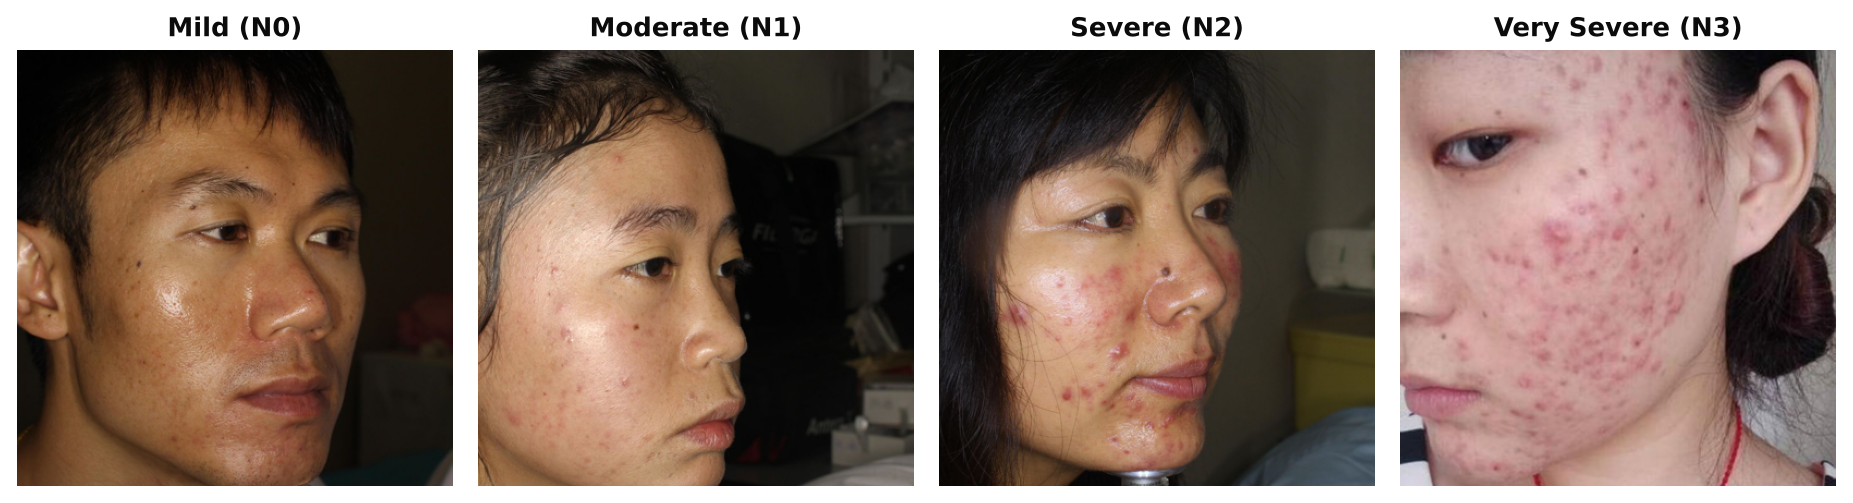
\includegraphics[width=\textwidth]{dataset_samples.png}
    \caption{Un exemple de photo pour chaque grade.}
    \label{fig:samples}
\end{figure}

\begin{table}[H]
    \centering
    \caption{Nombre de photos par grade.}
    \label{tab:dataset}
    \begin{tabular}{lrr}
        \toprule
        \textbf{Grade} & \textbf{Photos} & \textbf{Part} \\
        \midrule
        Mild (niveau 0)        & 483 & 35\% \\
        Moderate (niveau 1)    & 623 & 45\% \\
        Severe (niveau 2)      & 175 & 13\% \\
        Very Severe (niveau 3) &  96 &  7\% \\
        \midrule
        \textbf{Total}         & \textbf{1\,377} & 100\% \\
        \bottomrule
    \end{tabular}
\end{table}

\noindent Les classes sont \textbf{déséquilibrées} : il y a 6 fois plus de photos
\textit{Moderate} que de photos \textit{Very Severe}. Un modèle qui répondrait toujours
« Moderate » aurait déjà 45\% de bonnes réponses. C'est pourquoi nous jugeons le modèle
avec le \textbf{Macro-F1}, une mesure qui donne le même poids à chaque classe, et pas
seulement avec le pourcentage de bonnes réponses (\textit{accuracy}).

\section{Ce que nous a appris l'exploration des données}

Avant de construire le modèle, nous avons exploré les données dans le notebook
\texttt{notebooks/01\_eda.ipynb}. Les points principaux :
\begin{itemize}[noitemsep,topsep=4pt]
    \item Toutes les photos ont le même format (1024×1024, couleur, JPEG) : pas de nettoyage nécessaire.
    \item Les lésions sont \textbf{petites} : elles occupent une faible partie de la photo.
    \item Les photos \textit{Very Severe} sont en moyenne plus claires, à cause des conditions de prise de vue.
    \item Le dataset contient \textbf{36 paires de photos identiques}, dont 8 avec deux grades différents. Même les annotateurs hésitent parfois entre deux grades voisins.
\end{itemize}

\section{Les outils utilisés}

\begin{table}[H]
    \centering
    \caption{Les outils du projet et leur rôle.}
    \label{tab:outils}
    \begin{tabular}{>{\bfseries}l p{10.5cm}}
        \toprule
        \textbf{Outil} & \textbf{À quoi il sert} \\
        \midrule
        PyTorch      & Entraîner le réseau de neurones \\
        DVC          & Garder une version des données sans les mettre dans Git \\
        MLflow       & Enregistrer automatiquement chaque entraînement (réglages, scores, modèle) \\
        ONNX         & Convertir le modèle dans un format léger, utilisable sans PyTorch \\
        FastAPI      & Créer l'API qui reçoit une photo et renvoie la prédiction \\
        React        & Créer l'interface web \\
        Docker       & Emballer l'application pour qu'elle fonctionne partout pareil \\
        GitHub Actions & Lancer les tests automatiquement à chaque modification du code \\
        \bottomrule
    \end{tabular}
\end{table}

% ==============================================================================
\chapter{Préparation des données}

\section{Division en trois groupes}

Les photos sont réparties en trois groupes, chacun avec un rôle précis :
\begin{itemize}[noitemsep,topsep=4pt]
    \item \textbf{Entraînement (70\%, 963 photos)} : le modèle apprend à partir de ces photos ;
    \item \textbf{Validation (15\%, 205 photos)} : elles servent à choisir la meilleure version du modèle pendant l'entraînement ;
    \item \textbf{Test (15\%, 209 photos)} : elles sont mises de côté et utilisées \emph{une seule fois}, à la fin, pour mesurer la vraie performance.
\end{itemize}

\noindent La division est faite \textbf{grade par grade}, pour que chaque groupe garde les mêmes
proportions de classes (Figure~\ref{fig:distribution}). Elle utilise une graine aléatoire
fixe (42) : on obtient toujours exactement la même division. Elle est enregistrée dans
\texttt{data/processed/train.csv}, \texttt{val.csv} et \texttt{test.csv}.

\begin{figure}[H]
    \centering
    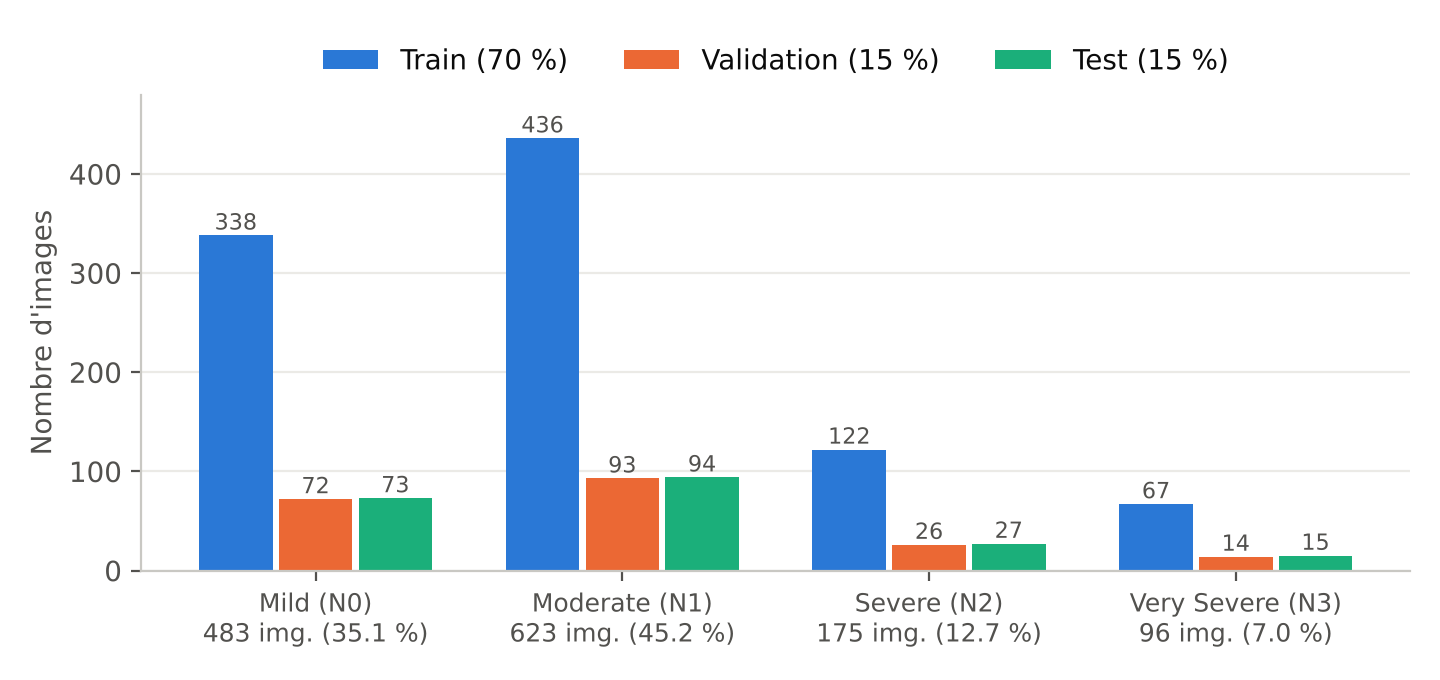
\includegraphics[width=0.85\textwidth]{class_distribution.png}
    \caption{Nombre de photos par grade dans chaque groupe.}
    \label{fig:distribution}
\end{figure}

\begin{resultatcle}
\textbf{Pourquoi c'est important (fuite de données)}

Si une photo de test a aussi été vue pendant l'entraînement, le score de test est
faussement bon. Nous avons donc :
\begin{itemize}[noitemsep,topsep=2pt]
    \item fait la division \emph{avant} toute transformation des photos ;
    \item vérifié que l'entraînement sur Kaggle a utilisé exactement la même division (963 / 205 photos) ;
    \item mesuré l'effet des photos en double du dataset : 4 photos de test ont une copie dans l'entraînement, mais sans elles le score reste le même (77,1\,\%).
\end{itemize}
\end{resultatcle}

\section{Transformations des photos}

Avant d'entrer dans le modèle, chaque photo est :
\begin{enumerate}[noitemsep,topsep=4pt]
    \item réduite de $1024\times1024$ à $224\times224$ pixels (la taille attendue par le modèle) ;
    \item normalisée avec les mêmes statistiques de couleur qu'ImageNet.
\end{enumerate}

\noindent Pour les photos d'\textbf{entraînement uniquement}, nous ajoutons des
modifications aléatoires : retournement gauche-droite et petite rotation ($\pm15^\circ$).
C'est l'\textbf{augmentation de données} : le modèle voit des variantes de chaque photo
et apprend mieux à généraliser. Les photos de validation et de test ne sont pas modifiées.

\section{Versionnement avec DVC}

Les 1\,377 photos (158 Mo) sont trop lourdes pour Git. \textbf{DVC} les stocke à part et met
dans Git un petit fichier, \texttt{data/raw/acne\_1024.dvc}, qui contient une empreinte
du dossier. Si une seule photo change, l'empreinte change. On sait donc toujours avec quelle
version des données un modèle a été entraîné.

\begin{lstlisting}[language=bash,caption={Commandes DVC principales.}]
dvc add data/raw/acne_1024    # suivre le dossier de photos
dvc push                      # envoyer les photos vers le stockage DVC
dvc pull                      # les récupérer sur une autre machine
\end{lstlisting}

% ==============================================================================
\chapter{Le modèle}

\section{Le transfer learning}

Entraîner un réseau de neurones à partir de zéro demande des centaines de milliers
d'images. Nous n'en avons que 1\,377. Nous utilisons donc le \textbf{transfer learning} :
nous partons d'un modèle déjà entraîné sur \textbf{ImageNet} (1,2 million d'images). Ce
modèle sait déjà reconnaître des formes, des textures et des contours. Il suffit de
l'adapter à notre problème.

\medskip
Le modèle choisi est \textbf{EfficientNet-B0}~\cite{tan2019efficientnet}, un réseau
convolutif (CNN) petit et rapide (4 millions de paramètres). Sa dernière couche, qui
reconnaissait 1\,000 catégories d'ImageNet, est remplacée par une couche à
\textbf{4 sorties}, une par grade.

\section{L'entraînement}

L'entraînement a été fait sur un \textbf{GPU gratuit de Kaggle}. Pendant 15 passages
complets sur les photos d'entraînement (\textit{époques}), le modèle prédit, mesure son
erreur et corrige ses poids. À la fin de chaque époque, il est évalué sur les photos de
validation, et la meilleure version est sauvegardée.

\begin{table}[H]
    \centering
    \caption{Réglages de l'entraînement.}
    \label{tab:hparams}
    \begin{tabular}{ll}
        \toprule
        \textbf{Réglage} & \textbf{Valeur} \\
        \midrule
        Modèle de départ & EfficientNet-B0 pré-entraîné sur ImageNet \\
        Époques & 15 \\
        Taille de lot (\textit{batch}) & 32 photos \\
        Taux d'apprentissage & 0,0001 \\
        Optimiseur & AdamW \\
        Choix du meilleur modèle & meilleur Macro-F1 en validation \\
        \bottomrule
    \end{tabular}
\end{table}

\begin{figure}[H]
    \centering
    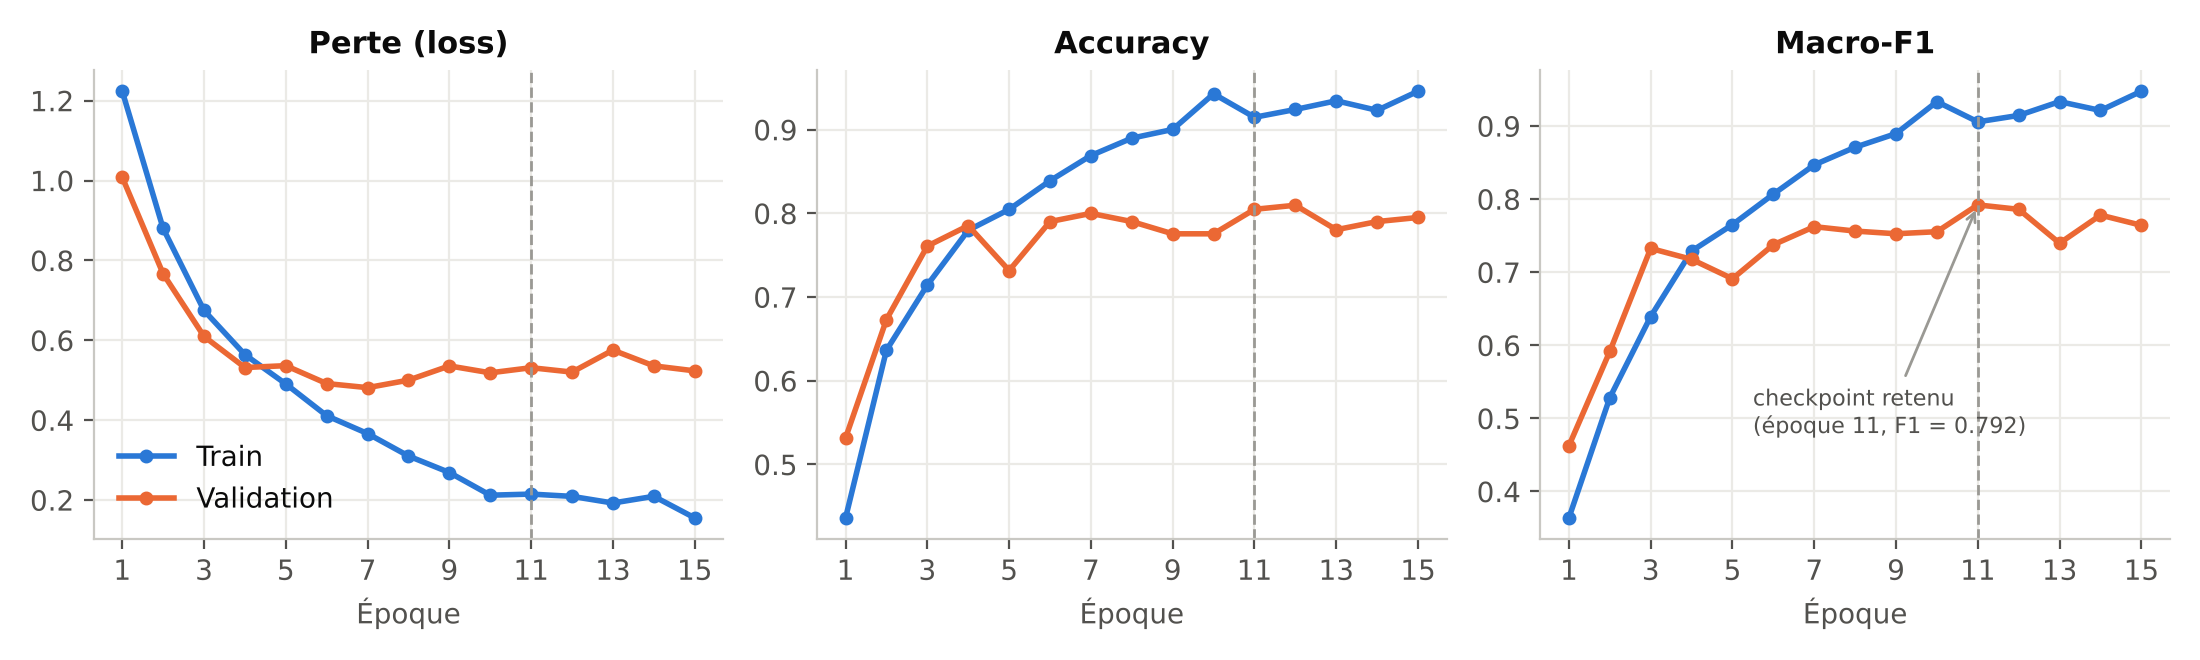
\includegraphics[width=\textwidth]{training_curves.png}
    \caption{Évolution de l'erreur (\textit{loss}), de l'accuracy et du Macro-F1 pendant l'entraînement.}
    \label{fig:curves}
\end{figure}

\noindent \textbf{Lecture des courbes :} sur les photos d'entraînement (en bleu), le modèle
s'améliore jusqu'à 95\% de bonnes réponses. Sur les photos de validation (en orange), il
plafonne autour de 80\%. Cet écart montre que le modèle commence à \textbf{apprendre par
cœur} les photos d'entraînement (\textit{sur-apprentissage}). La meilleure version est celle
de l'\textbf{époque 11} (Macro-F1 de validation : 0,79).

\section{La conversion en ONNX}

Le modèle entraîné est enregistré au format PyTorch. Pour l'utiliser dans l'API, nous le
convertissons au format \textbf{ONNX}. Ce format a deux avantages :
\begin{itemize}[noitemsep,topsep=4pt]
    \item l'API n'a pas besoin d'installer PyTorch, qui est très lourd ;
    \item la prédiction est rapide : environ \textbf{13 millisecondes} par photo sur un processeur normal.
\end{itemize}

\section{Réduire la taille du modèle}

Nous avons aussi créé deux versions plus légères du modèle, sans le réentraîner, en
stockant ses nombres avec moins de précision :

\begin{table}[H]
    \centering
    \caption{Les trois versions du modèle, testées sur les 209 photos de test.}
    \label{tab:quant}
    \begin{tabular}{lrrr}
        \toprule
        \textbf{Version} & \textbf{Taille} & \textbf{Accuracy} & \textbf{Macro-F1} \\
        \midrule
        Normale (32 bits, utilisée par l'API) & 16,0 Mo & 77,0\,\% & 0,73 \\
        16 bits (FP16) & 8,1 Mo & 77,0\,\% & 0,73 \\
        8 bits (INT8)  & 5,2 Mo & 72,7\,\% & 0,69 \\
        \bottomrule
    \end{tabular}
\end{table}

\noindent La version 16 bits est \textbf{deux fois plus petite sans aucune perte}. La version
8 bits est trois fois plus petite, mais perd 4 points de précision, car EfficientNet supporte
mal ce fort arrondi. Nous gardons donc la version normale dans l'application.

\section{Expliquer les décisions avec Grad-CAM}

Dans le domaine médical, il est important de comprendre \emph{pourquoi} un modèle donne
une réponse. Nous utilisons \textbf{Grad-CAM}~\cite{selvaraju2017gradcam}, une méthode
qui produit une \textbf{carte de chaleur} : les zones en rouge sont celles qui ont le plus
influencé la décision.

\begin{figure}[H]
    \centering
    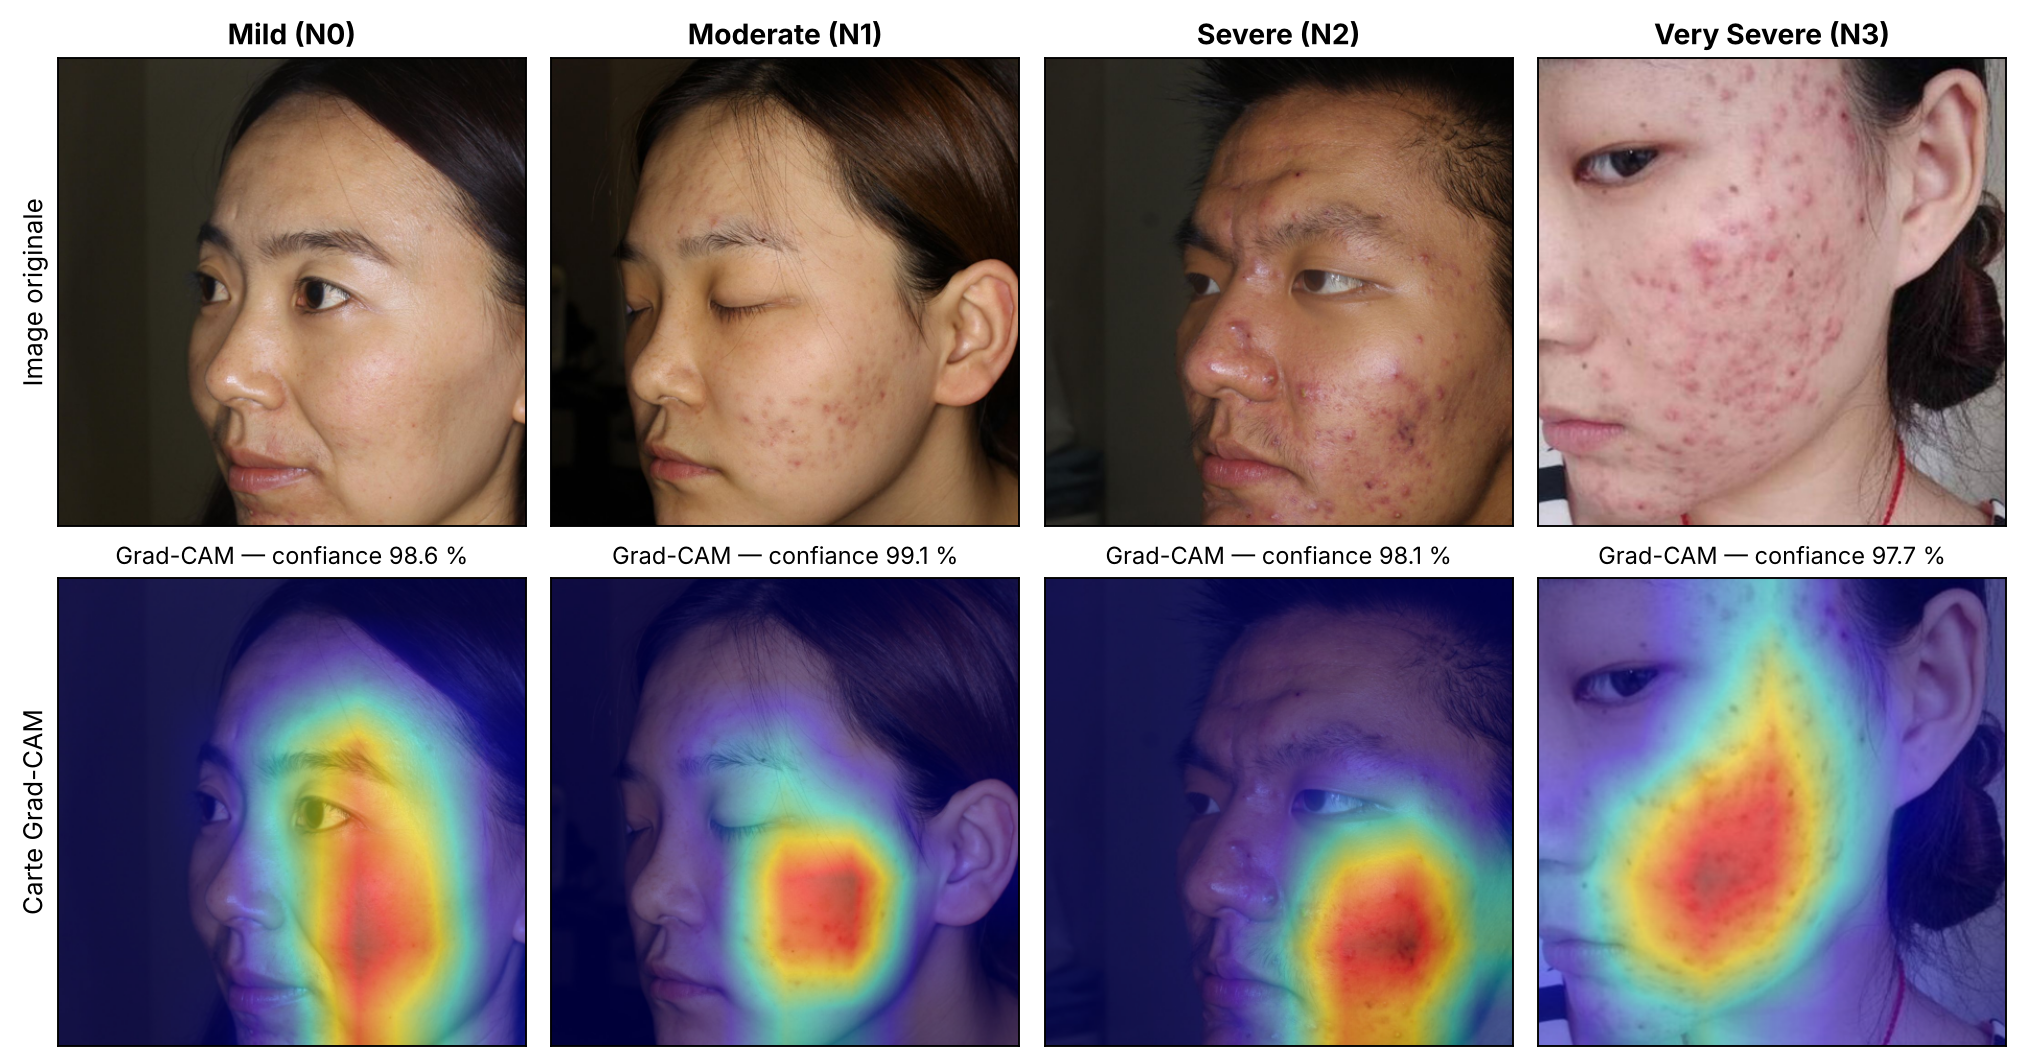
\includegraphics[width=\textwidth]{gradcam_grid.png}
    \caption{Cartes Grad-CAM de notre modèle sur des photos de test (une par grade).}
    \label{fig:gradcam}
\end{figure}

\noindent Dans l'application, cette carte est calculée directement à partir du modèle ONNX, sans PyTorch : elle fonctionne donc aussi dans Docker.

\medskip
\noindent Sur la Figure~\ref{fig:gradcam}, le modèle regarde bien les \textbf{joues et
les zones avec des boutons}, et pas l'arrière-plan. C'est un bon signe : il se base sur
la peau pour décider.

% ==============================================================================
\chapter{Résultats}

\section{Résultats principaux}

Le modèle final a été testé une seule fois sur les \textbf{209 photos de test}, qu'il n'avait
jamais utilisées pour apprendre.

\begin{resultatcle}
\textbf{Résultats sur les photos de test}
\begin{itemize}[noitemsep,topsep=2pt]
    \item \textbf{Accuracy : 77\,\%} (161 bonnes réponses sur 209)
    \item \textbf{Macro-F1 : 0,73}
    \item \textbf{Temps de prédiction : environ 13 ms} par photo
\end{itemize}
\end{resultatcle}

\section{Résultats par grade}

\begin{table}[H]
    \centering
    \caption{Résultats par grade sur les photos de test.}
    \label{tab:metrics}
    \begin{tabular}{lrrrr}
        \toprule
        \textbf{Grade} & \textbf{Précision} & \textbf{Rappel} & \textbf{F1} & \textbf{Photos} \\
        \midrule
        Mild (0)        & 0,80 & 0,84 & 0,82 &  73 \\
        Moderate (1)    & 0,79 & 0,79 & 0,79 &  94 \\
        Severe (2)      & 0,67 & 0,52 & 0,58 &  27 \\
        Very Severe (3) & 0,67 & 0,80 & 0,73 &  15 \\
        \bottomrule
    \end{tabular}
\end{table}

\noindent \textit{Précision} : quand le modèle annonce un grade, combien de fois il a raison.
\textit{Rappel} : parmi les photos d'un grade, combien le modèle en retrouve.
\textit{F1} : la moyenne des deux.

\medskip
Le grade \textbf{Severe} est le plus difficile (F1 = 0,58). Il y a peu de photos de ce grade
et il ressemble beaucoup à ses deux voisins.

\section{Matrice de confusion}

La matrice de confusion montre, pour chaque vrai grade (lignes), ce que le modèle a prédit
(colonnes). Les bonnes réponses sont sur la diagonale.

\begin{figure}[H]
    \centering
    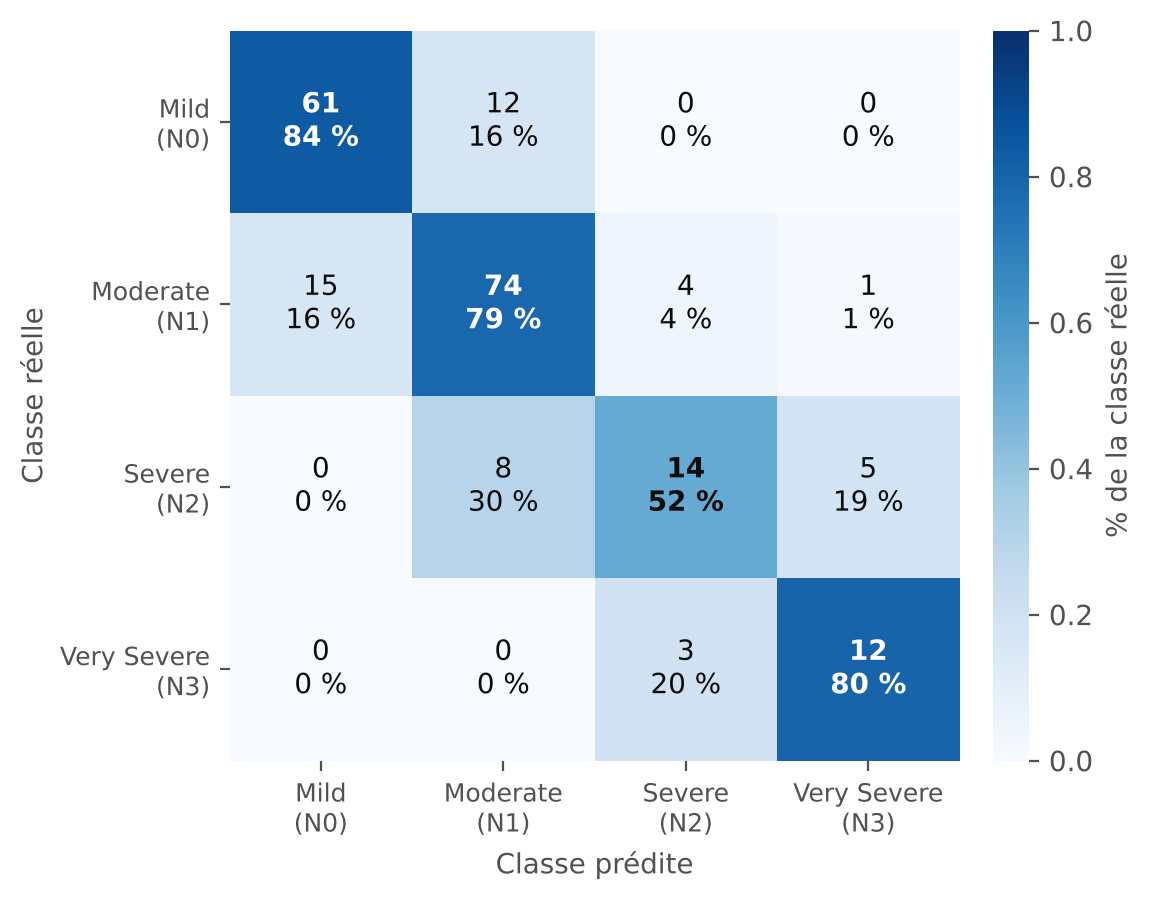
\includegraphics[width=0.6\textwidth]{confusion_matrix.png}
    \caption{Matrice de confusion sur les 209 photos de test.}
    \label{fig:cm}
\end{figure}

\noindent Presque toutes les erreurs (\textbf{47 sur 48}) se font entre deux \textbf{grades
voisins}, par exemple \textit{Severe} prédit comme \textit{Moderate}. Le modèle ne confond
jamais une acné légère avec une acné sévère. Ces erreurs sont compréhensibles : les
annotateurs du dataset eux-mêmes ont parfois donné deux grades voisins à la même photo.

\section{Comparaison avec un modèle de référence}

Pour vérifier que notre choix d'EfficientNet-B0 est bon, nous avons entraîné un
\textbf{modèle de référence} (\textit{baseline}) : \textbf{ResNet-18}, un réseau classique plus
ancien. Tout le reste est identique : mêmes photos, mêmes réglages, même nombre d'époques. Seul
le modèle change.

\begin{table}[H]
    \centering
    \caption{Modèle de référence contre modèle choisi (photos de test).}
    \label{tab:baseline}
    \begin{tabular}{lrr}
        \toprule
        & \textbf{ResNet-18 (référence)} & \textbf{EfficientNet-B0} \\
        \midrule
        Taille du modèle & 44,7 Mo & \textbf{16,0 Mo} \\
        Accuracy         & 75,6\,\% & \textbf{77,0\,\%} \\
        Macro-F1         & 0,67 & \textbf{0,73} \\
        Grade \textit{Very Severe} retrouvé & 5 sur 15 & \textbf{12 sur 15} \\
        Temps de prédiction & 20,5 ms & \textbf{10,2 ms} \\
        \bottomrule
    \end{tabular}
\end{table}

\begin{figure}[H]
    \centering
    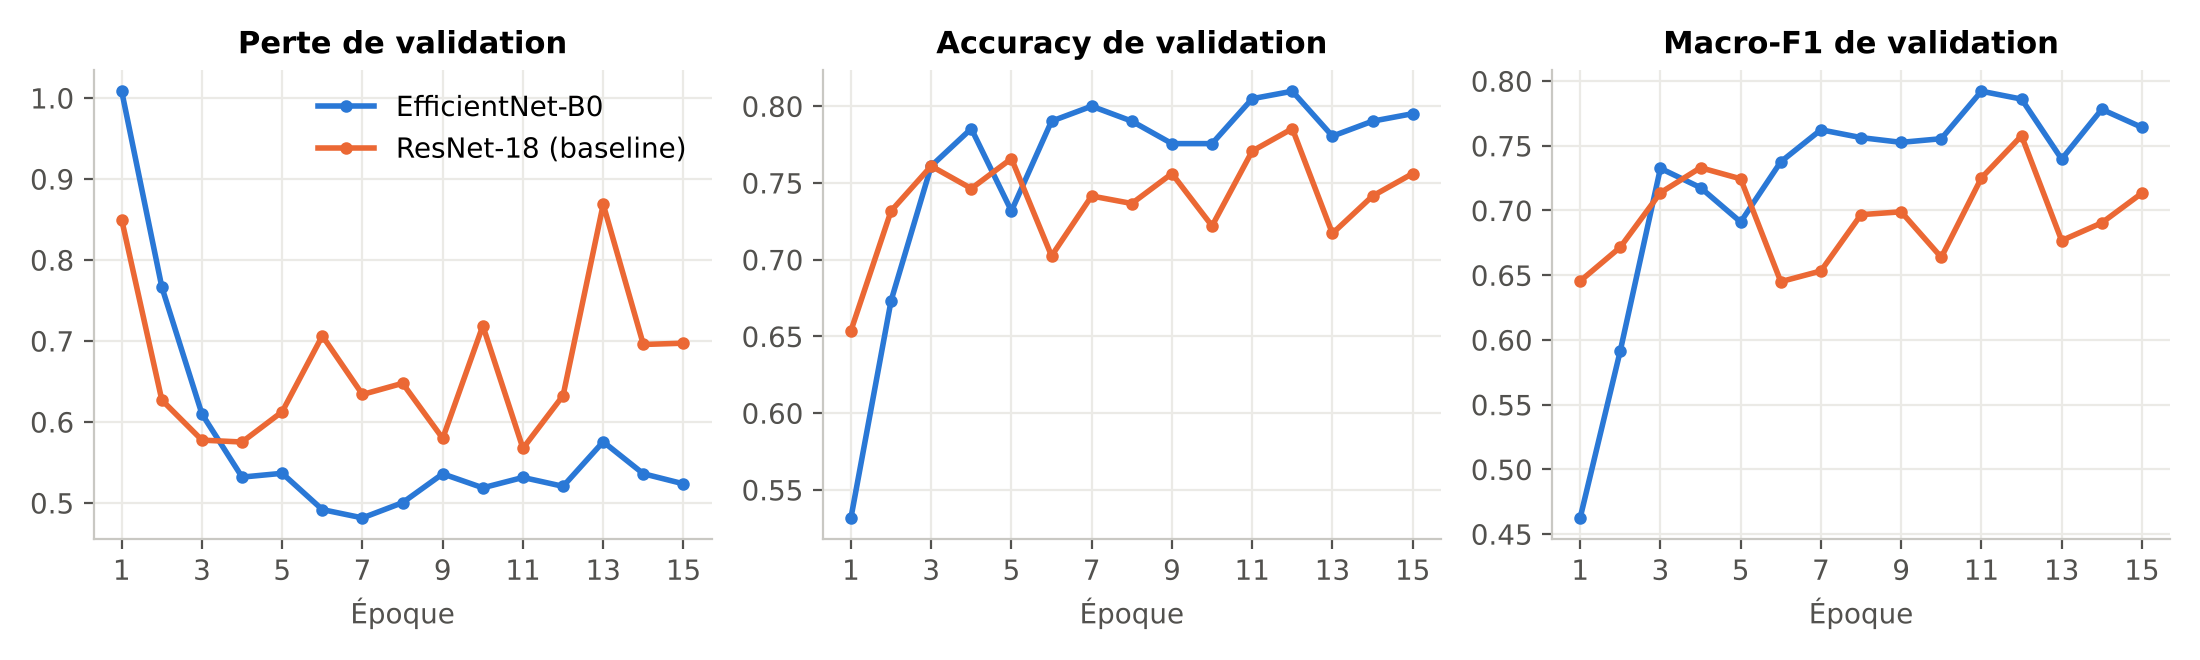
\includegraphics[width=\textwidth]{baseline_vs_efficientnet.png}
    \caption{Évolution des deux modèles pendant l'entraînement (photos de validation).}
    \label{fig:baseline_curves}
\end{figure}

\noindent EfficientNet-B0 est \textbf{meilleur sur tous les points}, tout en étant presque
trois fois plus petit et deux fois plus rapide. La différence la plus nette concerne le grade
rare \textit{Very Severe}. Les deux entraînements sont enregistrés dans MLflow, ce qui permet de
les comparer côte à côte.

\section{Comparaison avec la littérature et limites}

Dans l'article original d'ACNE04~\cite{wu2019acne04}, un modèle CNN classique (ResNet-50)
obtient environ 78\% et la meilleure méthode des auteurs 84\%. Notre résultat (77\% avec
un modèle plus petit) est donc proche d'un CNN classique, mais pas encore au niveau de
l'état de l'art.

\begin{limite}
\textbf{Limites actuelles}
\begin{itemize}[noitemsep,topsep=2pt]
    \item Le modèle sur-apprend : 95\% sur l'entraînement contre 80\% en validation.
    \item Le grade \textit{Severe} est souvent confondu avec \textit{Moderate}.
    \item En réduisant les photos à 224 pixels, les petits boutons deviennent flous.
    \item Avec seulement 209 photos de test, le score a une marge d'erreur d'environ $\pm6$ points.
\end{itemize}
\end{limite}

% ==============================================================================
\chapter{L'application et les outils MLOps}

\section{Architecture générale}

L'application est séparée en plusieurs parties indépendantes (Figure~\ref{fig:architecture}).
En haut, ce qui tourne quand on utilise l'application ; en bas, ce qui sert à créer le modèle.

\begin{figure}[H]
    \centering
    \begin{tikzpicture}[
        box/.style={draw=darkblue!70, fill=resultbg, rounded corners=3pt, minimum height=1.15cm,
                    minimum width=3.1cm, align=center, font=\small},
        arr/.style={-{Stealth[length=2.5mm]}, thick, darkblue!80},
        lab/.style={font=\scriptsize, text=black!65, align=center},
        node distance=1.2cm and 2.1cm]
      \node[box] (user) {\textbf{Utilisateur}\\navigateur web};
      \node[box, right=of user] (front) {\textbf{Interface}\\React\\(port 5173)};
      \node[box, right=of front] (api) {\textbf{API}\\FastAPI\\(port 8000)};
      \node[box, below=1.9cm of user] (dvc) {\textbf{Données}\\ACNE04 + DVC};
      \node[box, right=of dvc] (train) {\textbf{Entraînement}\\PyTorch (Kaggle)\\+ MLflow};
      \node[box, right=of train] (onnx) {\textbf{Modèle}\\fichier ONNX};
      \draw[arr, <->] (user) -- node[lab, above]{clic,\\photo} (front);
      \draw[arr, <->] (front) -- node[lab, above]{envoi /\\réponse} (api);
      \draw[arr] (dvc) -- (train);
      \draw[arr] (train) -- node[lab, above]{export} (onnx);
      \draw[arr] (onnx) -- node[lab, right]{chargé par l'API} (api);
      \begin{scope}[on background layer]
        \node[draw=black!25, dashed, rounded corners, fit=(user)(front)(api), inner sep=8pt,
              label={[font=\scriptsize\itshape, text=black!55]above:Utilisation (Docker Compose)}] {};
        \node[draw=black!25, dashed, rounded corners, fit=(dvc)(train)(onnx), inner sep=8pt,
              label={[font=\scriptsize\itshape, text=black!55]below:Création du modèle}] {};
      \end{scope}
    \end{tikzpicture}
    \caption{Les différentes parties de SkinWise AI.}
    \label{fig:architecture}
\end{figure}

\section{Ce qui se passe quand on analyse une photo}

\begin{enumerate}[topsep=4pt]
    \item L'utilisateur dépose une photo, en prend une avec la webcam, ou clique sur l'un des 4 exemples de la galerie.
    \item L'interface envoie la photo à l'API (\texttt{POST /predict}).
    \item L'API vérifie que c'est bien une image, la réduit à 224 pixels et la donne au modèle ONNX.
    \item Le modèle renvoie un pourcentage pour chacun des 4 grades.
    \item L'interface demande la carte Grad-CAM (\texttt{POST /predict/visualize}).
    \item Elle affiche le grade, la confiance, les 4 pourcentages, la carte de chaleur et deux temps : le calcul du modèle sur le serveur, et le temps total mesuré par le navigateur (Figure~\ref{fig:ui}).
\end{enumerate}

\begin{figure}[H]
    \centering
    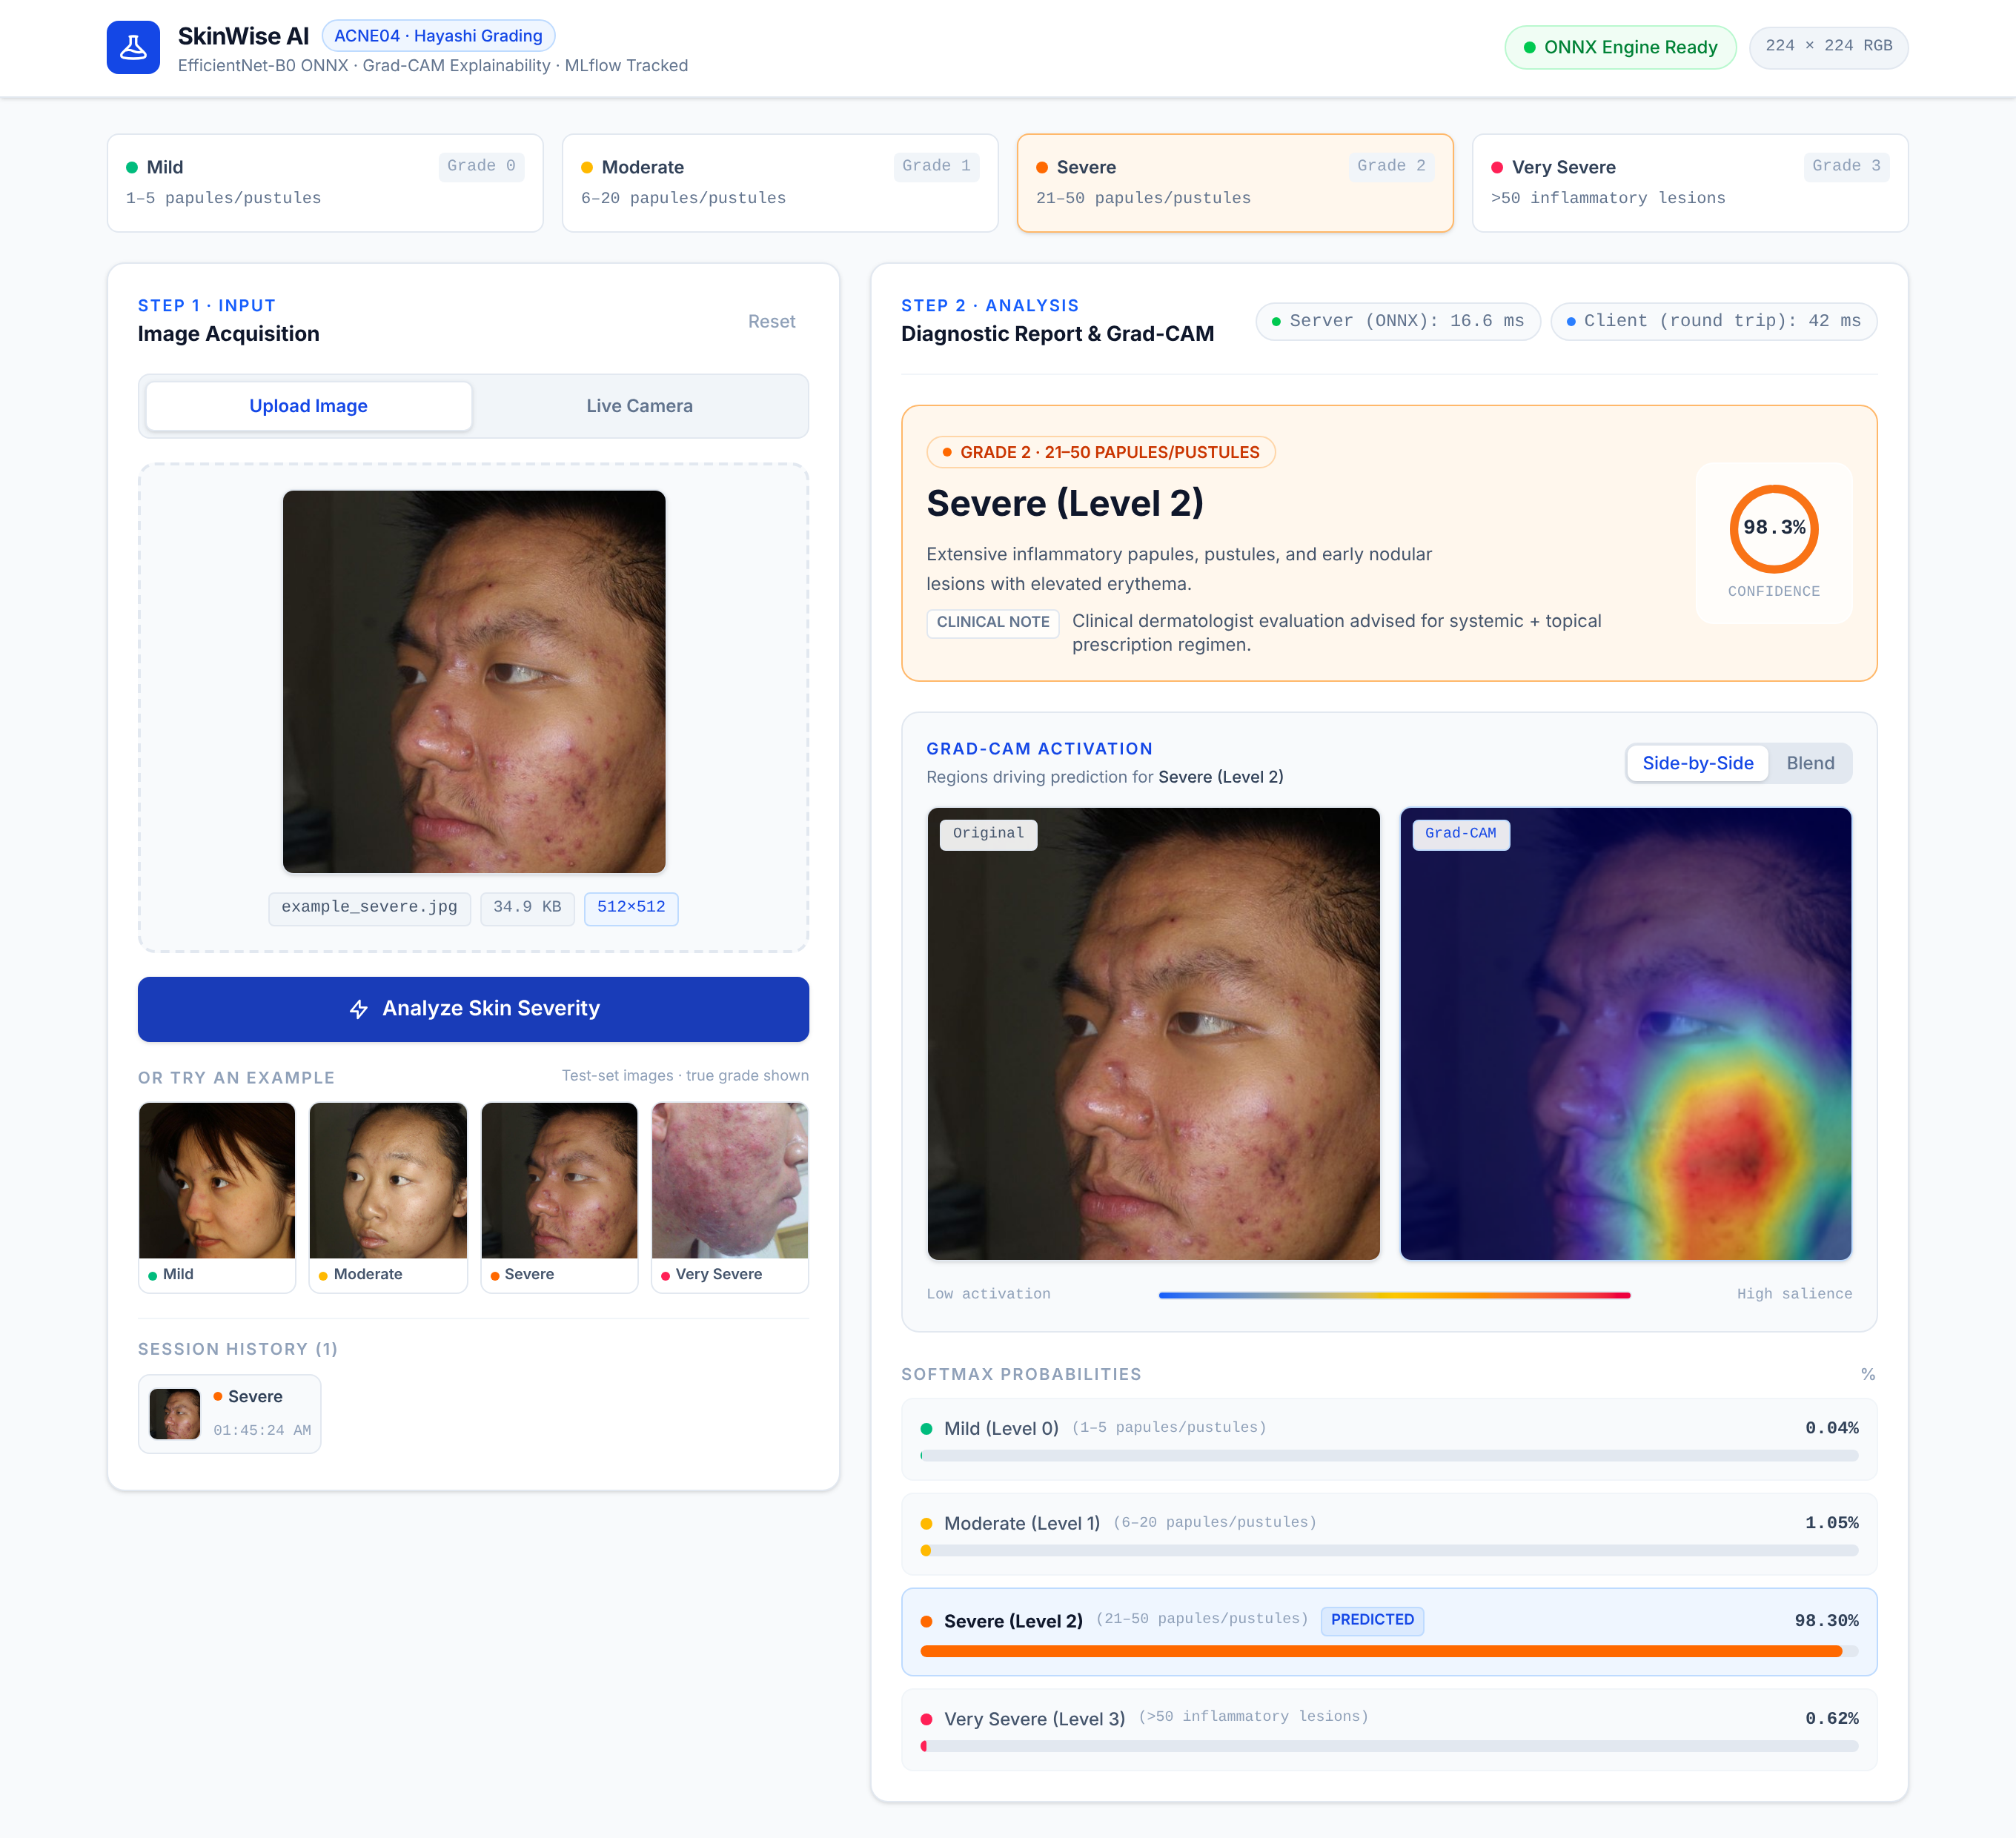
\includegraphics[width=0.92\textwidth]{ui_result.png}
    \caption{L'interface après un clic sur l'exemple \textit{Severe} de la galerie (en bas à gauche).}
    \label{fig:ui}
\end{figure}

\section{L'API}

L'API est faite avec \textbf{FastAPI}. Elle propose quatre adresses :

\begin{table}[H]
    \centering
    \caption{Les adresses de l'API.}
    \label{tab:api}
    \begin{tabular}{ll}
        \toprule
        \textbf{Adresse} & \textbf{Rôle} \\
        \midrule
        \texttt{GET /health}            & Vérifier que le serveur marche et que le modèle est chargé \\
        \texttt{GET /model/metadata}    & Donner les informations du modèle (nom, classes) \\
        \texttt{POST /predict}          & Recevoir une photo et renvoyer le grade prédit \\
        \texttt{POST /predict/visualize}& Renvoyer la carte de chaleur Grad-CAM \\
        \bottomrule
    \end{tabular}
\end{table}

\noindent Les réponses suivent un format strict défini avec \textbf{Pydantic}. Si on envoie
un fichier qui n'est pas une image, l'API répond avec une erreur claire (code 400). FastAPI
génère aussi automatiquement une page de documentation interactive (Figure~\ref{fig:swagger}).

\begin{figure}[H]
    \centering
    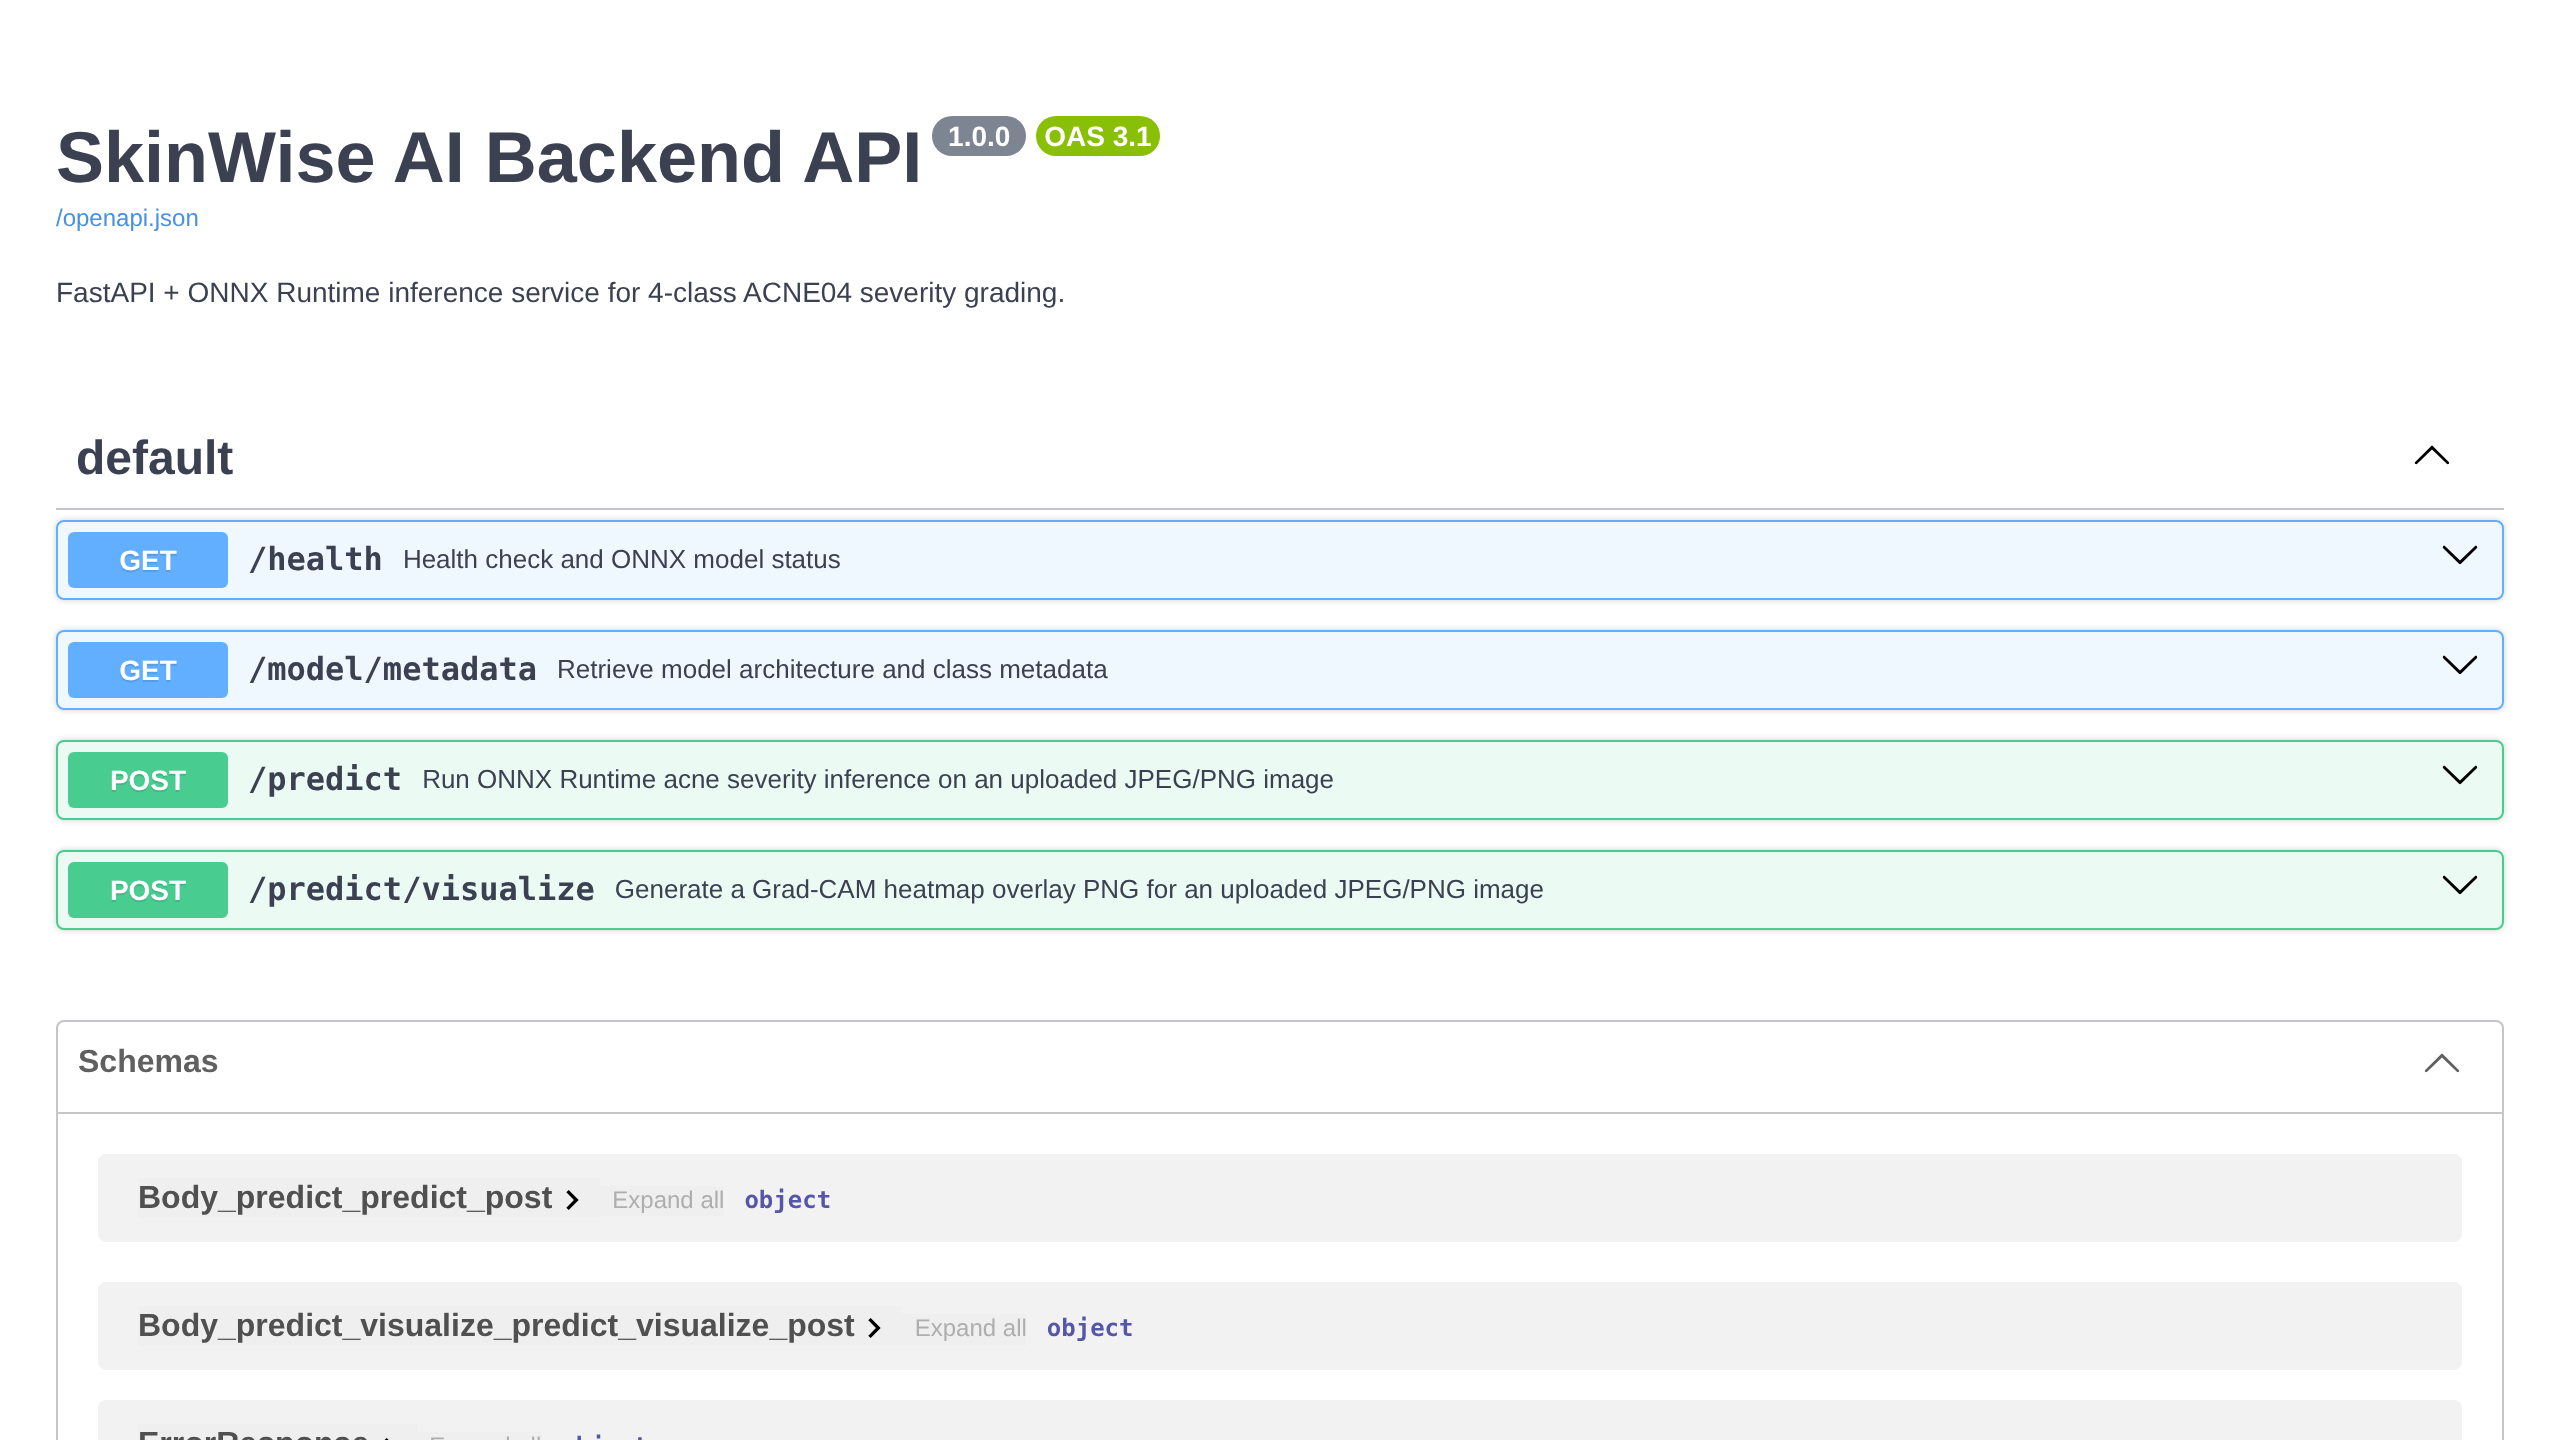
\includegraphics[width=0.85\textwidth]{swagger.png}
    \caption{Page de documentation automatique de l'API (\texttt{http://localhost:8000/docs}).}
    \label{fig:swagger}
\end{figure}

\section{Suivi des expériences avec MLflow}

À chaque entraînement, \textbf{MLflow} enregistre automatiquement les réglages, les scores de
chaque époque et le modèle obtenu. On peut ainsi comparer les essais et retrouver
n'importe quel ancien modèle. Le meilleur modèle est enregistré dans le
\textbf{Model Registry} avec le statut \textbf{Production} (Figure~\ref{fig:mlflow}).

\begin{figure}[H]
    \centering
    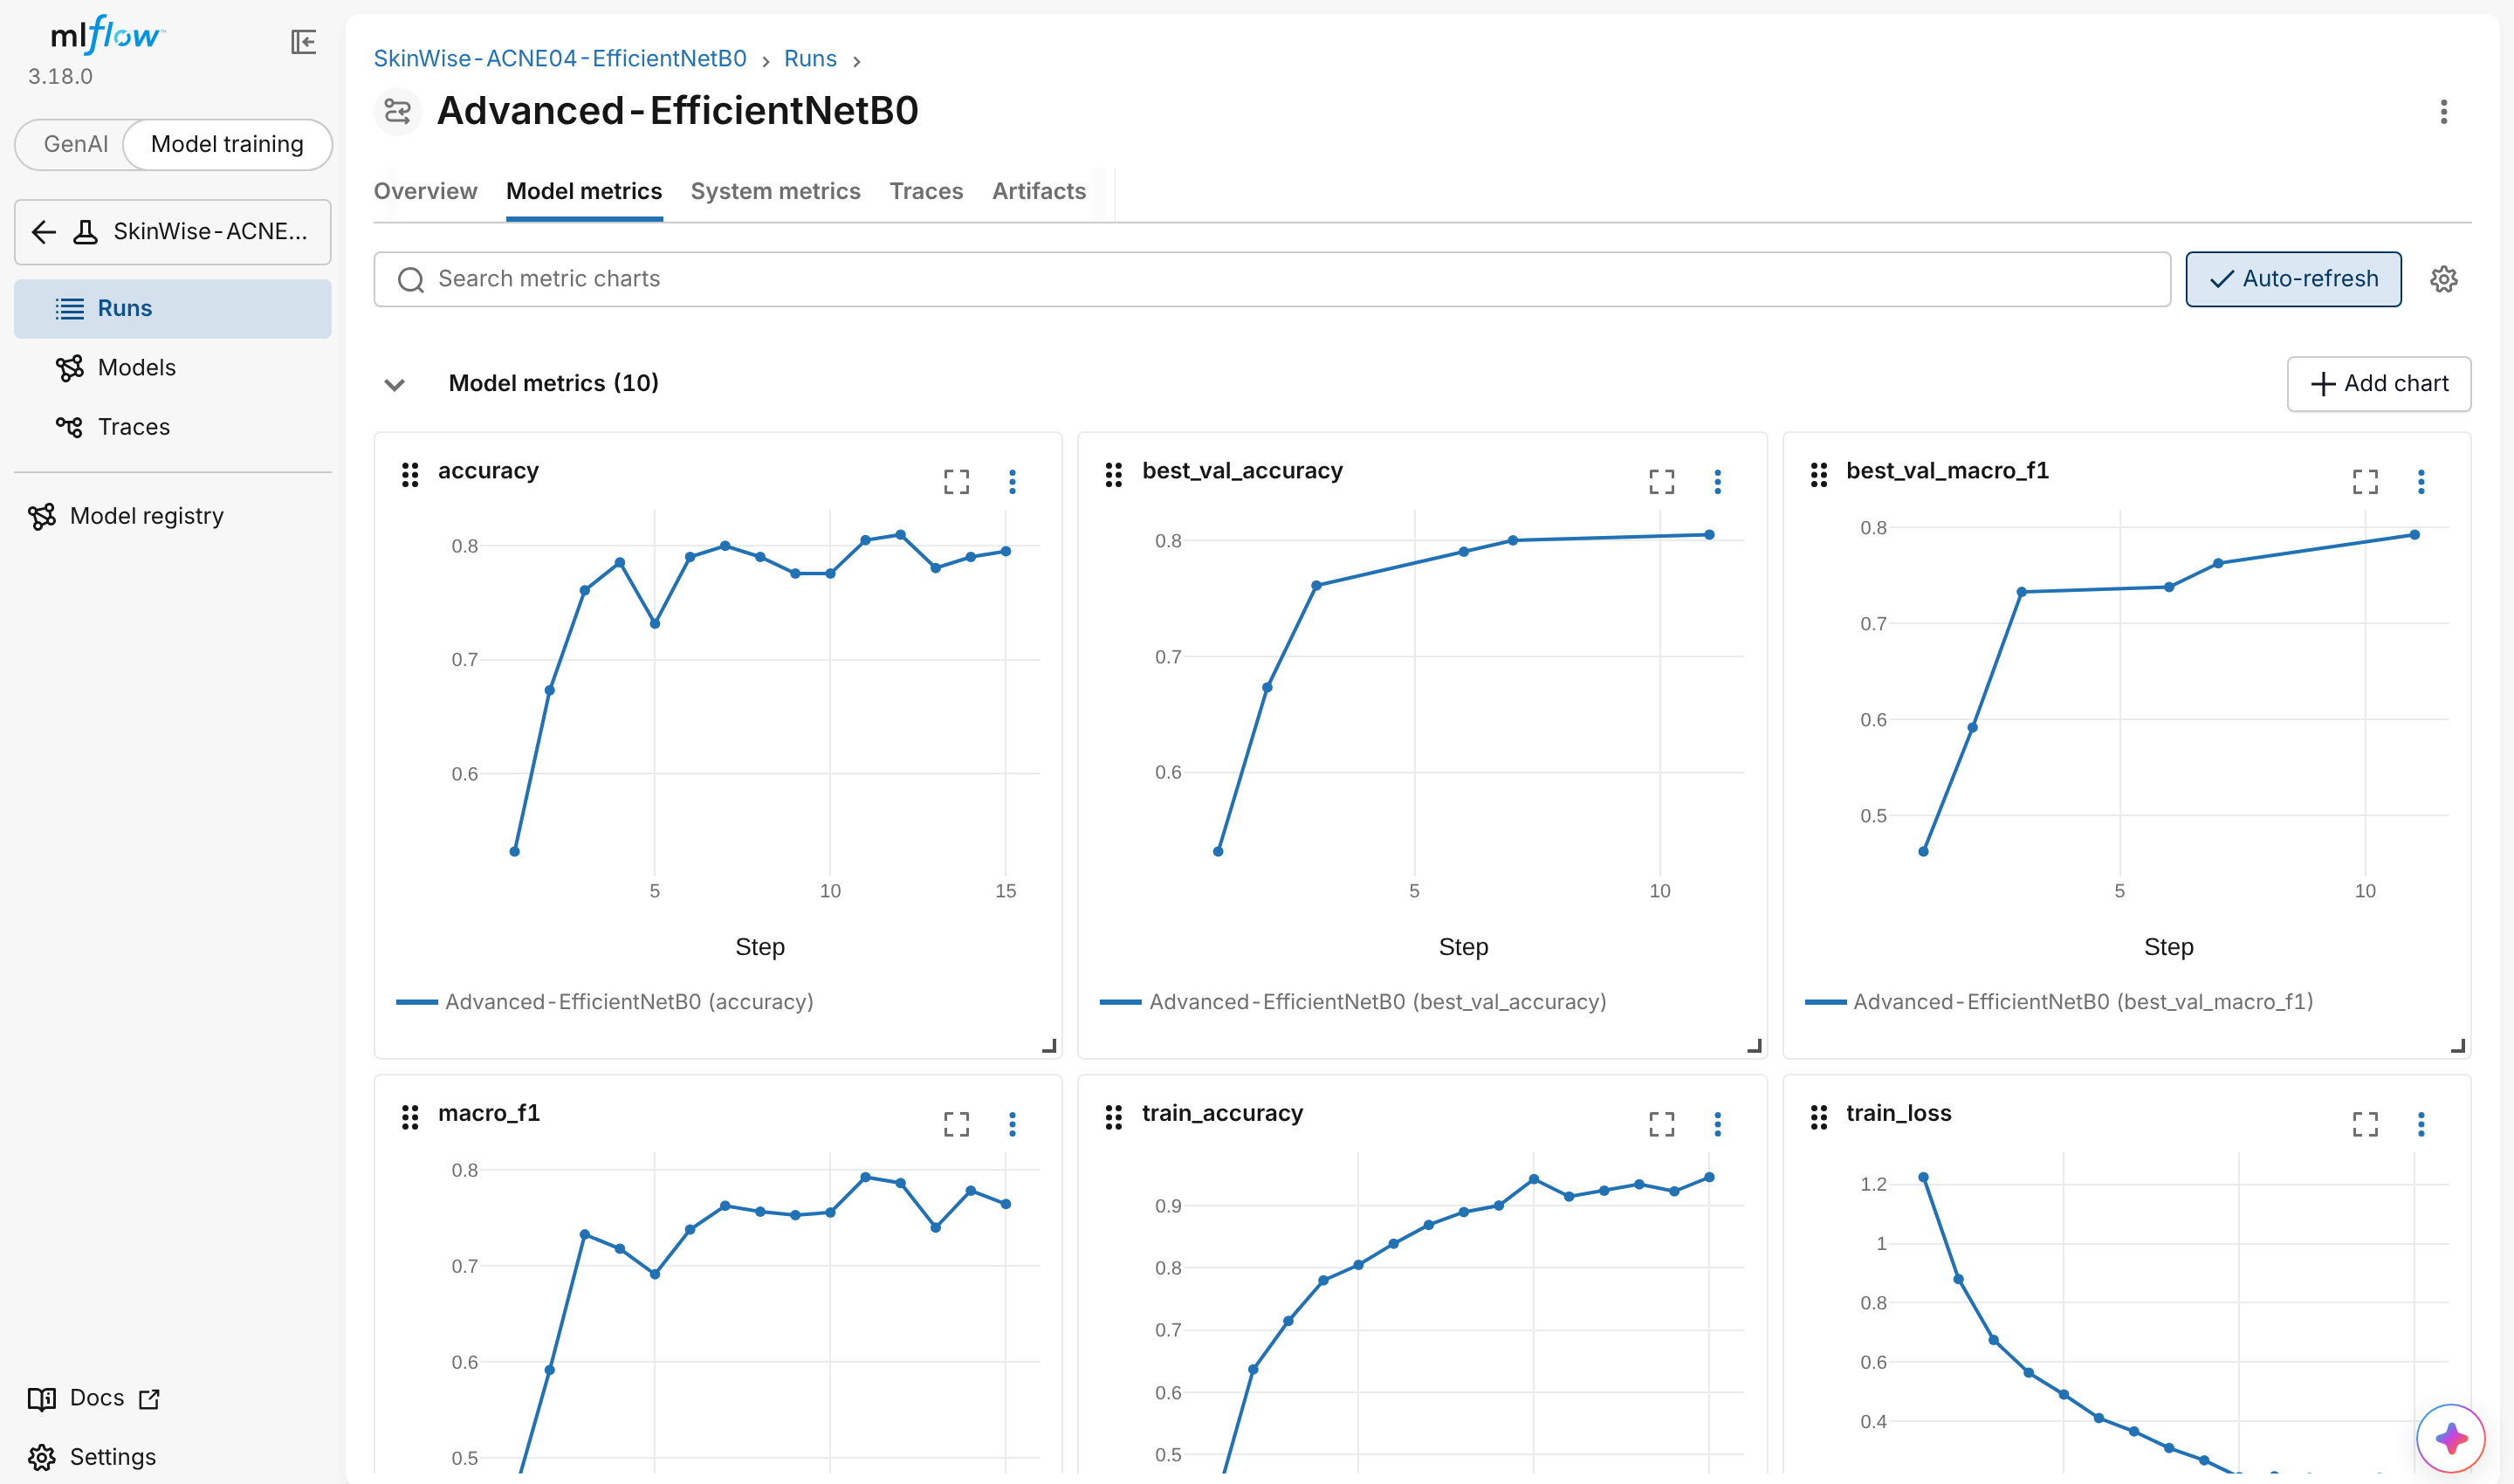
\includegraphics[width=\textwidth]{mlflow_metrics.png}
    \caption{MLflow : les scores enregistrés à chaque époque.}
    \label{fig:mlflow}
\end{figure}

\begin{figure}[H]
    \centering
    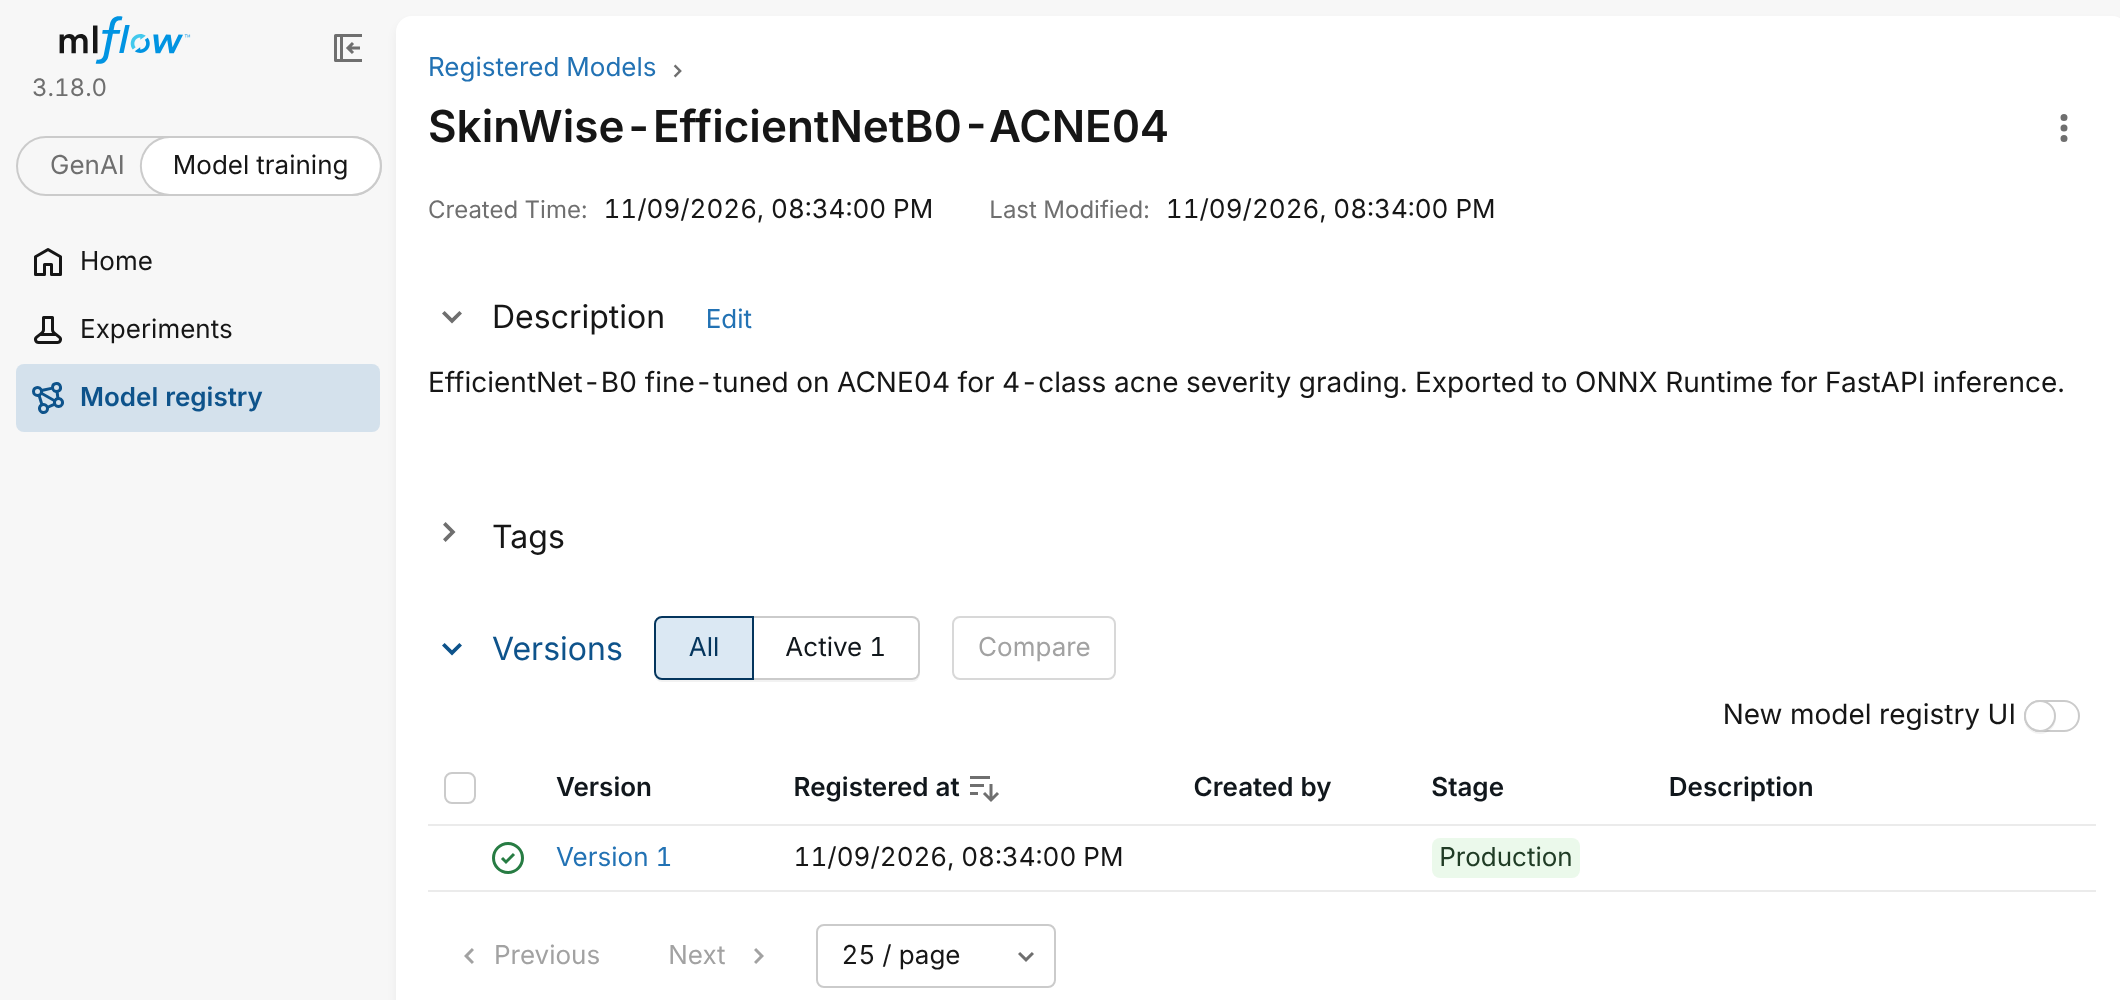
\includegraphics[width=0.75\textwidth]{mlflow_registry.png}
    \caption{MLflow Model Registry : le modèle en statut \textit{Production}.}
    \label{fig:registry}
\end{figure}

\section{Docker : lancer l'application en une commande}

\textbf{Docker} met l'API et l'interface chacune dans un « conteneur » qui contient tout ce
dont elle a besoin. L'application fonctionne donc de la même façon sur n'importe quel
ordinateur. L'interface est servie par \textbf{nginx}, un serveur web rapide, et l'API tourne
sans les options de développement. \textbf{Docker Compose} lance les deux conteneurs ensemble :

\begin{lstlisting}[language=bash,caption={Lancer toute l'application.}]
docker-compose up --build
# Interface : http://localhost:5173
# API       : http://localhost:8000/docs
\end{lstlisting}

\section{Tests automatiques avec GitHub Actions}

À chaque envoi de code sur GitHub, \textbf{GitHub Actions} lance automatiquement :
\begin{itemize}[noitemsep,topsep=4pt]
    \item une vérification du style du code Python (\texttt{flake8}) et JavaScript (\texttt{ESLint}) ;
    \item 16 tests (\texttt{pytest}) de l'API et des fonctions de prédiction, par exemple : « un fichier texte doit être refusé », « une image valide doit recevoir 4 pourcentages dont la somme fait 100\,\% » ;
    \item la construction des images Docker et un test de démarrage de l'application.
\end{itemize}

\noindent Si un test échoue, GitHub l'affiche en rouge avant que le code ne soit intégré.

\section{Organisation des fichiers}

\begin{lstlisting}[caption={Les dossiers principaux du projet.}]
SkinWise/
|-- data/            les photos (raw/) et la division train/val/test (processed/)
|-- notebooks/       l'exploration des données (01_eda.ipynb)
|-- src/             le code du modèle : données, entraînement, évaluation, Grad-CAM
|-- models/          le modèle entraîné (.pth et .onnx)
|-- backend/         l'API FastAPI et ses tests
|-- frontend/        l'interface React
|-- .github/         les tests automatiques (GitHub Actions)
|-- dvc.yaml         les étapes du pipeline DVC
|-- docker-compose.yml   le lancement de l'application
`-- README.md        le guide d'installation
\end{lstlisting}

% ==============================================================================
\chapter*{Conclusion}
\addcontentsline{toc}{chapter}{Conclusion}
\markboth{Conclusion}{Conclusion}

Nous avons réalisé \textbf{SkinWise AI}, une application complète qui prédit le grade de
sévérité de l'acné à partir d'une photo et explique sa décision avec une carte de chaleur.

\medskip
Le modèle, un EfficientNet-B0 adapté par transfer learning, obtient \textbf{77\,\% de bonnes
réponses} et un \textbf{Macro-F1 de 0,73} sur des photos qu'il n'avait jamais utilisées pour
apprendre. Presque toutes ses erreurs se font entre deux grades voisins. Il fait mieux qu'un
modèle de référence (ResNet-18) entraîné dans les mêmes conditions, tout en étant trois fois plus
petit.

\medskip
Autour du modèle, nous avons mis en place les bonnes pratiques MLOps demandées : versions
des données avec DVC, suivi des entraînements avec MLflow, modèle léger avec ONNX, API
FastAPI, interface React, conteneurs Docker et tests automatiques avec GitHub Actions.

\medskip
\textbf{Pistes d'amélioration :}
\begin{enumerate}[noitemsep,topsep=4pt]
    \item Utiliser des images plus grandes (384 pixels) pour mieux voir les petits boutons.
    \item Réduire le sur-apprentissage avec plus d'augmentation de données (MixUp, CutMix).
    \item Mieux traiter les grades rares (Focal Loss, poids par classe).
    \item Retirer les photos en double du dataset avant la division.
    \item Rendre la version 8 bits aussi précise que la normale (entraînement adapté à la quantification).
\end{enumerate}

% ==============================================================================
\begin{thebibliography}{9}
\bibitem{wu2019acne04}
X.~Wu, N.~Wen, J.~Liang et al.,
``Joint Acne Image Grading and Counting via Label Distribution Learning,''
\textit{ICCV}, 2019.

\bibitem{tan2019efficientnet}
M.~Tan and Q.~V.~Le,
``EfficientNet: Rethinking Model Scaling for Convolutional Neural Networks,''
\textit{ICML}, 2019.

\bibitem{selvaraju2017gradcam}
R.~R.~Selvaraju et al.,
``Grad-CAM: Visual Explanations from Deep Networks via Gradient-based Localization,''
\textit{ICCV}, 2017.
\end{thebibliography}

\end{document}
